Scopo dell'esperienza è la determinazione sperimentale dell'indice di rifrazione dell'acqua utilizzando la legge di Snell:

\begin{equation}
	n = \frac{\sin(\Theta_i)}{\sin(\Theta_r)}
\end{equation}

Per svolgere questo esperimento è stato utilizzato un semplice setup costituito da una vaschetta di plastica trasparente con carta millimetrata visibile sul fondo, un'asta con un'altezza superiore a quella della vaschetta e una riga. L'asta ci ha permesso di mantenere fissa la posizione di osservazione, fissando l'occhio ad una distanza costante dal fondo.

\begin{figure}[H]
	\centering
	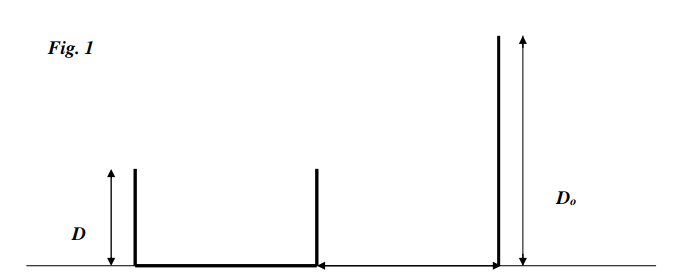
\includegraphics[width=0.75\textwidth]{./figures/Im1}
	\caption{La figura mette in relazione l'altezza $D$ della vaschetta e l'altezza $D_0$ dell'asta.}
\end{figure}

\begin{figure}[H]
	\centering
	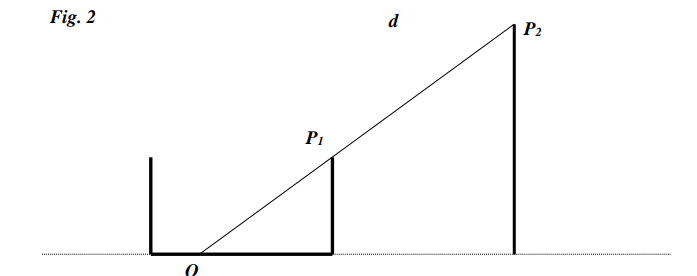
\includegraphics[width=0.75\textwidth]{./figures/Im2}
	\caption{Il punto $P_2$, posto ad una data altezza dell'asta, rappresenta il punto fisso da cui sono state effettuate le osservazioni. Il punto $P_1$ rappresenta la cima della vaschetta. A vaschetta vuota, La direzione individuata dai punti $P_2$ e $P_1$ permette di determinare il punto $O$ di intersezione tra la retta passante per i punti $P_1$ e $P_2$ ed il fondo della vaschetta.}
\end{figure}

Determinato il punto $O$, l'esperimento prosegue col progressivo riempimento della vaschetta. Versando dell'acqua all'interno della vaschetta, e sia $h$ il suo livello, guardando ancora nella direzione $P_1\ P_2$, per effetto della rifrazione, non verrà più visualizzato il punto $O$ ma l'immagine $O'$ come mostrato in Figura (3).

\begin{figure}[H]
	\centering
	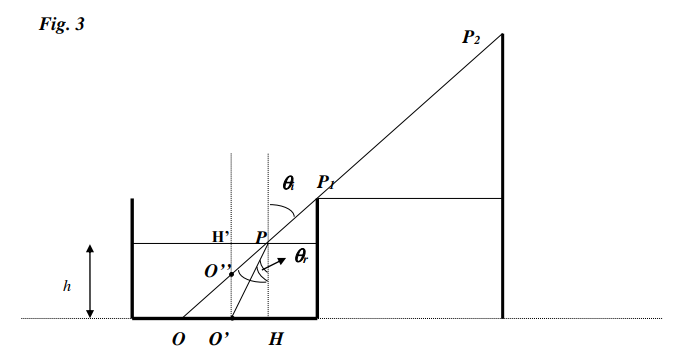
\includegraphics[width=0.75\textwidth]{./figures/Im3}
	\caption{In figura è mostrato l'effetto della rifrazione dovuto alla presenza di un generico liquido all'interno della vaschetta, il cui livello è $H'$ e il suo angolo di rifrazione $\Theta_r$. In figura è anche rappresentato l'angolo di incidenza $\Theta_i$.}
\end{figure}

La distanza $OO'$, che sarà indicata con $x$, al variare del livello dell'acqua $h$ segue un andamento lineare, in particolare: 

\begin{equation}
	x=h(\tan(\Theta_i)-\tan(\Theta_r))
\end{equation}}

Riportando in grafico $x$ in funzione di $h$ è possibile calcolare l'angolo di rifrazione $\Theta_r$ dal coefficiente angolare della retta di regressione. A questo punto, tramite la Legge (1), si ottiene l'indice di rifrazione.

